\section{Animation Physics}

Animation is about creating the illusion of motion, e.g. by rapidly displaying of a sequence of static images that minimally differ from each other. There are three basic techniques to animate motion in computers:
\begin{itemize}
	\item Artist Directed, e.g. using keyframes
	\item Data Driven, e.g. motion capture
	\item Procedural, e.g. simulation
\end{itemize}


\subsection{Key Framing}

The idea behind key framing is to specify important events only, computer fills in the rest via interpolation or approximation. We also call this event and they do not have to be position, it could also be color, lighting, etc. \medskip

How do we interpolate data? Linear interpolation is simple but yields rather rough motion. A more appropriate interpolation technique would be to use spline interpolation.

\subsection{Splines}

In general, a spline is any piecewise polynomial function defined by data points $(t_i, f_i)$, so that $f(t_i) = f_i$. The only other condition is that the function is a polynomial when restricted to any interval between knots. \medskip

Most commonly we use cubic splines (degree three). As cubic polynomials have four degrees of freedom, there are multiple solutions to interpolate given points. To find a solutions we need further restrictions, so we match the derivatives at the endpoints.

\subsubsection{Natural Splines}

Piecewise spline made up of cubic polynomials $p_i$.
\begin{center}
	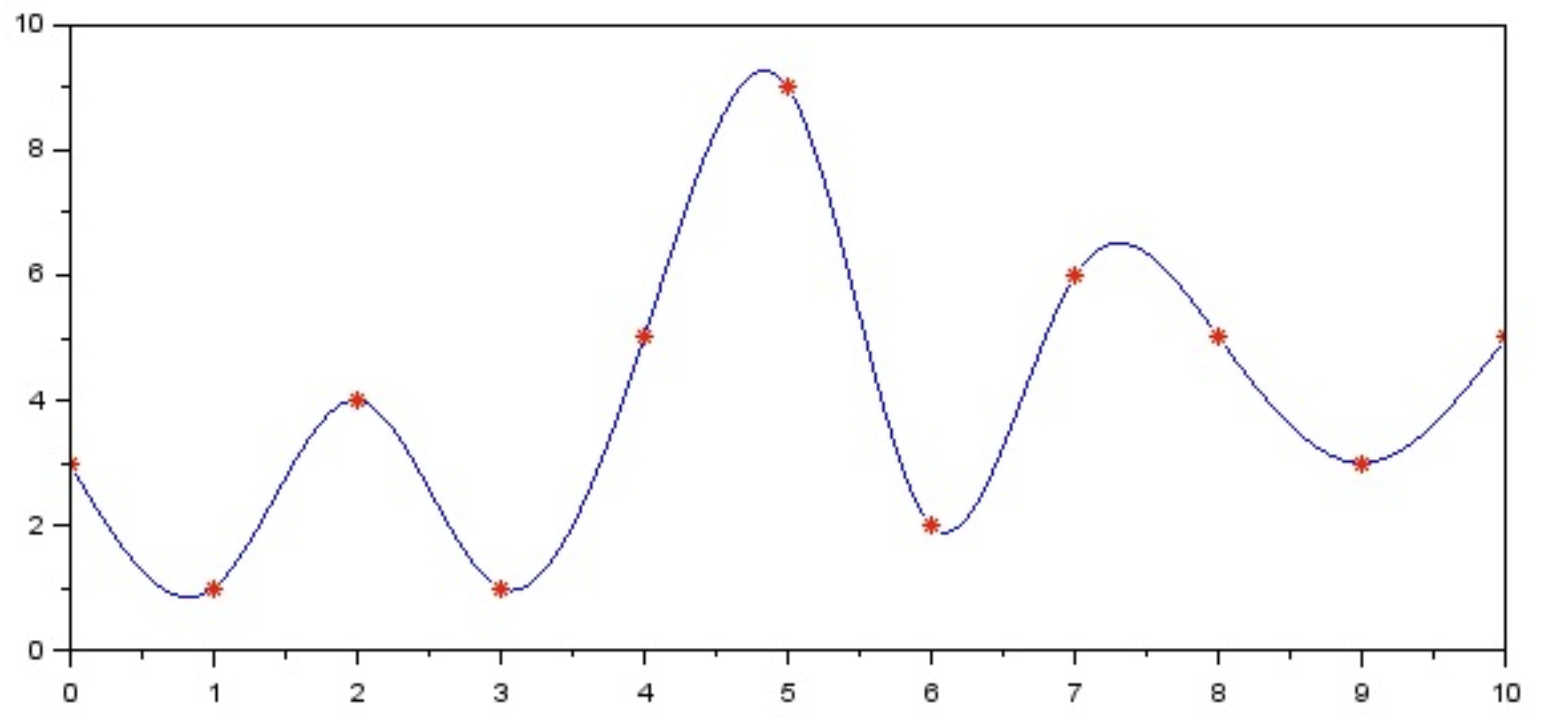
\includegraphics[width=\linewidth]{natural_spline.png}
\end{center}

We want that these polynomials are $C^2$ continuous at the knots. This leaves us with two degrees of freedom remaining, so we have to introduce conditions for the endpoints. We set the curvature to zero at endpoints, therefore we can solve this system. \medskip

This function now interpolates the data and is $C^2$ continuous everywhere, but there is still a problem. If we move one knot, it will have an influence on the whole curve (locality).

\subsubsection{Hermite / Bezier Splines}

We have already seen B-Splines, they fulfil the locality condition but the $C^2$ continuity is gone. For each knot we have to additionally specify the tangents. These type of splines are the most used in computer graphics and animation.

\subsubsection{Catmull-Rom Splines}

Sometimes makes sense to specify tangents, but often it is more convenient to just specify values. Catmull-Rom splines are a specialization of Hermite splines, determined by values alone. They use difference of neighbors to define the tangents. Commonly they are used to interpolate motion in computer animation.
